\documentclass{report}
\usepackage[utf8]{inputenc}
\usepackage[spanish]{babel}
\usepackage{graphicx}


\title{Vectorizado de siluetas por algoritmos genéticos}
\author{Adrián Arroyo Calle}
\date{ Octubre-Noviembre 2017}
\begin{document}

\maketitle

\chapter{Introducción}
En el mundo gráfico existen dos tipos fundamentales de imágenes.
En primer lugar tenemos las rasterizadas, donde se almacena la información de cada píxel.
Estas imágenes son las generadas por escáneres y cámaras fotográficas, así como por renders
de ordenador. Los formatos más usados son JPEG y PNG. En segundo lugar tenemos las imágenes
vectoriales, donde se almacenan funciones matemáticas. Este tipo de imágenes son muy usadas
en ilustraciones, diseño gráfico y videojuegos. Los formatos más usados son SVG y AI. 

Para obtener una imagen rasterizada desde una imagen vectorial, el procedimiento es
sencillo. Simplmente se aplican las fórmulas matemáticas sobre un lienzo de un determinado
tamaño. En cambio, el procedimiento inverso es extremadamente complicado. 

El algoritmo genético presentado en este documento permite transformar imágenes rasterizadas
sencillas en imágenes vectoriales.

\chapter{Estructura general}

El procedimiento básico que seguirá el programa, que será implementado en el lenguaje 
de programación Rust\cite{Matsakis:2014:RL:2692956.2663188}, será el siguiente:

\begin{enumerate}
	\item Leer imagen rasterizada de entrada
	\item Pasar la imagen a escala de grises
	\item Detección de esquinas en la imagen
	\item Optimización de las conexiones entre esquinas
	\item Salida de la imagen vectorial
\end{enumerate}

Para los 3 primeros pasos usaremos librerías de código abierto disponibles para Rust. Concretamente
usaremos image e imageproc. Esta última contiene los algoritmos de detección de esquinas FAST9 y 
FAST12. Sin embargo posteriormente se comprobó que ambos algoritmos tenían tasas de acierto
demasiado bajas y por ello se permite la edición manual de las esquinas.

Será en el paso 4 es donde se aplicará el algoritmo genético, ya que se trata de una tarea de 
optimización. Los algoritmos genéticos pueden ser aplicados de forma exitosa en problemas donde 
necesitemos optimizar algo. En nuestro caso, queremos optimizar el trazado de una línea a que 
respete la forma original sobre la que se está dibujando. Esta línea será una curva cúbica de Bézier.

Finalmente el último paso se realizará de forma trivial por nosotros mismos, 
exportando la imagen a SVG.

\chapter{Detección de esquinas}
La librería imageproc contiene los algoritmos de detección de esquinas
FAST9 y FAST12 \cite{rosten_2006_machine} (acrónimo de Features from accelerated segment test). 
Estos algoritmos, son mucho más rápidos que el
 famoso algoritmo de Harris-Stephens, ofreciendo una calidad aceptable, aunque no suficiente para 
 nuestro algoritmo de vectorización. Un ejemplo de su funcionamiento lo podemos ver en la 
 figura \ref{fig:fast-png}.

 % EXPLICAR FAST

\section{Interfaz de usuario}

Debido a la baja tasa de aciertos de FAST9 y FAST12 en las imágenes de prueba, se permite también
añadir puntos de forma manual. Para ello se ha diseñado una interfaz gráfica en GTK3, gracias a
la librería gtk-rs que permite usar GTK en Rust. La interfaz fue diseñada en Glade. La interfaz, 
que se aprecia en la figura \ref{fig:interfaz}, 
es muy sencilla. El funcionamiento principal es con el ratón. Cuando se hace click izquierdo en un
lugar de la imagen se añade una esquina. Cuando se hace click derecho, esa esquina se elimina. 
Además hay varios botones en el lateral derecho. Un botón para aplicar FAST9 a la imagen \ref{fig:fast9}, otro para eliminar 
todas las esquinas y otro para ejecutar el algoritmo.

\begin{figure}
	\center{
		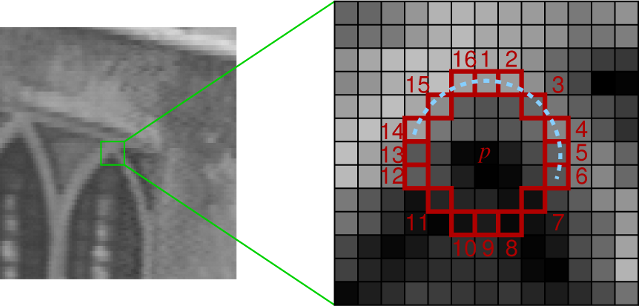
\includegraphics[width=\textwidth]{fast.png}
	}
	\caption{\label{fig:fast-png} Ejemplo de ejecución de FAST sobre una imagen}
\end{figure}

\begin{figure}
	\center{
		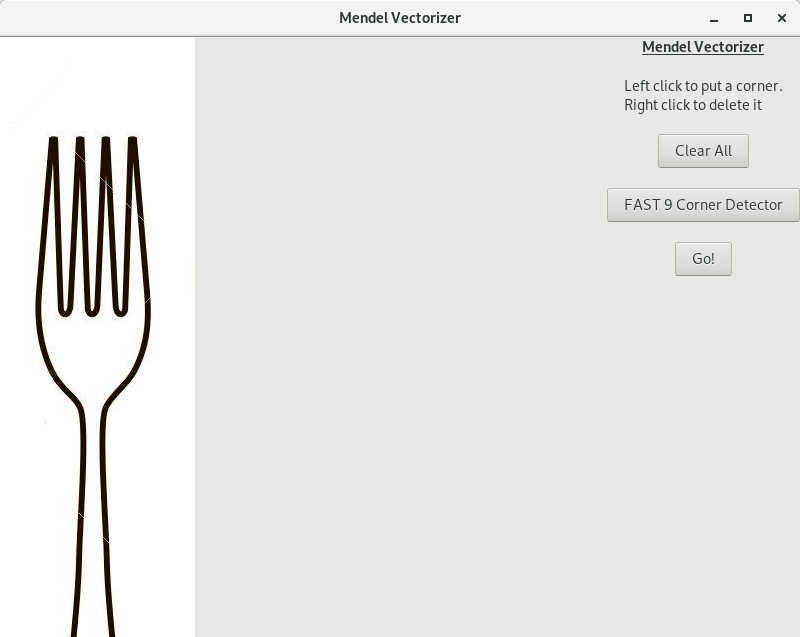
\includegraphics[width=\textwidth]{interfaz-usuario.png}
	}
	\caption{\label{fig:interfaz} Interfaz de usuario para seleccionar esquinas}
\end{figure}

\begin{figure}
	\center{
		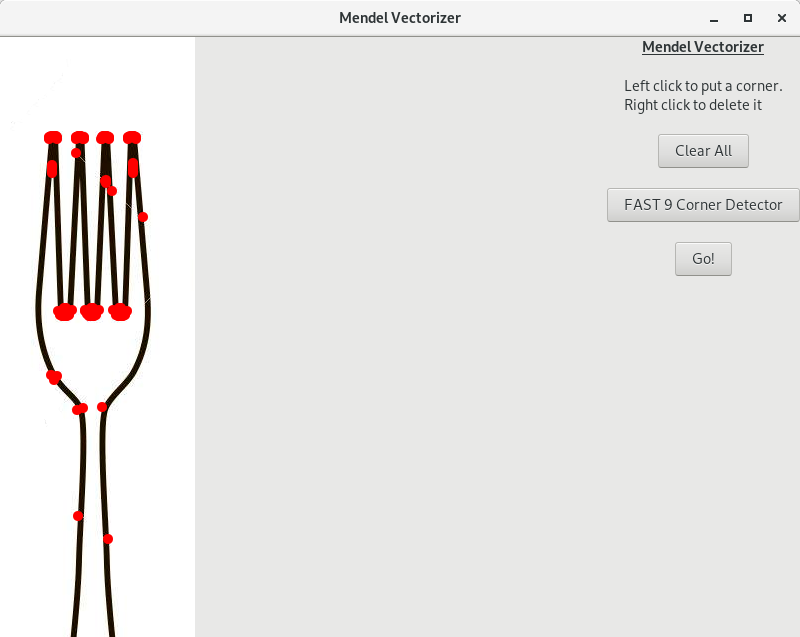
\includegraphics[width=\textwidth]{fast9.png}
	}
	\caption{\label{fig:fast9} Ejemplo de ejecución de FAST9 en la interfaz de usuario}
\end{figure}

\chapter{Algoritmo genético}

Los algoritmos genéticos son aquellos que se basan en el concepto de la evolución biológica.
En estos algoritmo se crea una muestra con parámetros aleatorios y se evalúa su desempeño.
Los peores son eliminados y los mejores sufren mutaciones aleatorias. Así de forma repetitiva hasta
llegar a tener una muestra con parámetros suficientemente buenos como para resolver el problema de 
forma casi óptima.

\section{Curva cúbica de Bézier}

El algoritmo en esencia trata de encontrar una línea que una dos puntos, de forma lo más parecida
posible a una imagen dada. Estas líneas en nuestro caso van a ser siempre curvas cúbicas de Bézier,
un subtipo de spline muy usado en gráficos por ordenador.\cite{wiki:bezier}

Estas curvas se basan en dos puntos de inicio y final y dos puntos de control, que permiten controlar
la curva con facilidad, véase la figura \ref{fig:bezier}.

\begin{figure}
	\center{
		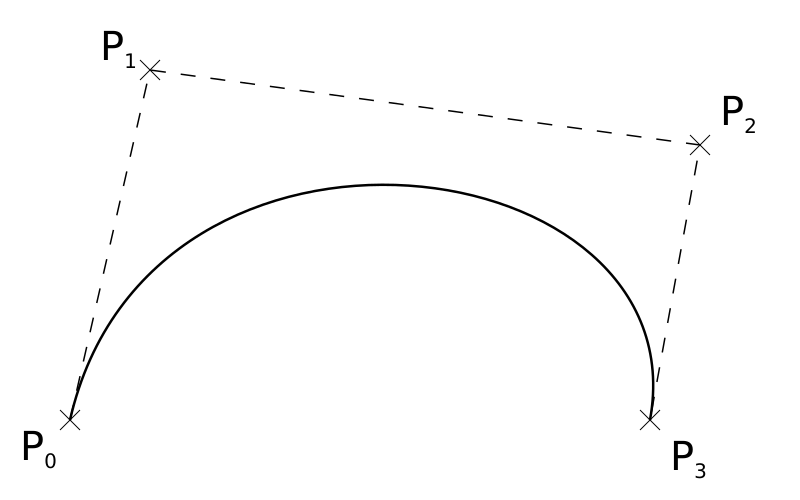
\includegraphics[width=\textwidth]{bezier.png}
	}
	\caption{\label{fig:bezier} Curva cúbica de Bézier}
\end{figure}

La forma paramétrica de una curva cúbica de Bézier es la siguiente:  \\

\begin{math}
	\mathbf{B}(t)=\mathbf{P}_0(1-t)^3+3\mathbf{P}_1t(1-t)^2+3\mathbf{P}_2t^2(1-t)+\mathbf{P}_3t^3 \mbox{ , } t \in [0,1].
\end{math}



\section{Función de evaluación}

Un ingrediente fundamental del algoritmo genético es la función de evaluación, que mide cuán buena
es la solución dada por un individuo. Nuestra función de evaluación toma la curva cúbica de Bezier y 
calcula
los puntos en 100 lugares de la curva. Estos puntos se comparan con la imagen real, si ahí había una línea
se suma un punto, si no, se resta.

\section{Análisis de coste}



\bibliography{memoria}
\bibliographystyle{acm}
\nocite{*}

\end{document}
